% subseccion 4.1  
\subsection{Fase 1: Planeación}\label{sec:planeacion}
En esta etapa se estableció el propósito general para el SMS y se definieron los objetivos del estudio, preguntas de investigación, métricas, tópicos de clasificación, criterios de inclusión y exclusión y criterios de calidad. Ver Figura \ref{fig:PlanningStageOverview}.
Para los componentes ``Objetivos del estudio'', ``Preguntas de investigación'' y ``Métricas'', de la etapa de planificación, se aplicó el modelo {\itshape Goal-Question-Metric} (GQM por sus siglas en inglés) \cite{basili1992software, caldiera1994goal}. Estos componentes consideran el nivel conceptual, operacional y cuantitativo, respectivamente según Sepulveda et al. \cite{Sepúlveda202141}.

\begin{figure}[htbp]
	\centering
	\vspace{10pt}
	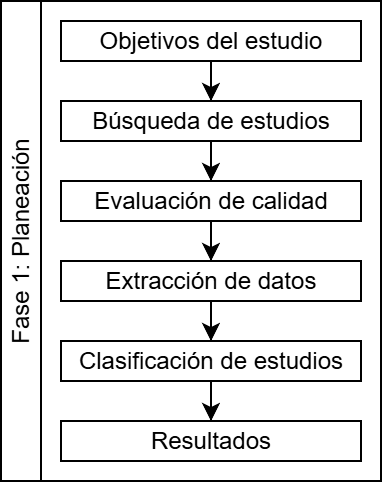
\includegraphics[scale=0.7]{resources/figures/sms-Etapa-1 overview.drawio.png}
	\vspace{6pt}
	\caption{Componentes de la etapa de planeación.}
	\label{fig:PlanningStageOverview}
\end{figure}

% 4.1.1
%sub-subseccion - objetivos del estudio
\subsubsection{Objetivos del estudio}
Teniendo en cuenta los aspectos descritos en la sección de motivación, se han definido dos objetivos para el estudio, detallados en la Tabla \ref{table:Goals}.

\begin{table}[htbp]

	\centering
	\renewcommand{\arraystretch}{1.7}  % Espaciado entre filas
	\setlength{\tabcolsep}{3pt}      % Espaciado horizontal en celdas
	\vspace{10pt}                     % Espacio arriba de la tabla (opcional)
	\begin{tabular}{|>{\arraybackslash}m{1cm}|>{\arraybackslash}m{7cm}|}
		\hline
		\textbf{Objetivo} & \textbf{Descripción}                                                                                                                                                                                                                                                                                                                                         \\
		\hline
		G1                & Clasificar trabajos relacionados con los universos de HTCondor según su aplicación e impacto en los dominios de computación distribuida y paralela, HTC, desarrollo de Software, virtualización y microservicios, redes de computadoras, infraestructura computacional, inteligencia artificial, análisis de datos y pensamiento computacional, entre otros. \\
		\hline
		G2                & Identificar y categorizar trabajos vinculados con los universos de HTCondor como herramienta para fortalecer funciones esenciales universitarias como: investigación, docencia, extensión e industria.                                                                                                                                                       \\
		\hline
	\end{tabular}
	\vspace{6pt}  % Espacio entre tabla y caption
	\caption{Objetivos del SMS.}
	\label{table:Goals}

\end{table}

% 4.1.2
%sub-subseccion - pregunta de investigación
\subsubsection{Pregunta de investigación}
Para la construcción de las preguntas de investigación (RQ por sus siglas en inglés) se usó el modelo PICOC \cite{Needleman20026, Petticrew2008systematic}, que nos permite establecer los aspectos ``Población'', ``Intervención'', ``Comparación'', ``Resultados'' y ``Contexto''. Todo esto para situar el trabajo en un entorno adecuado y propender por la entrega de valor. Ver Tabla \ref{table:PICOC}.

\begin{table}[htbp]

	\centering
	\renewcommand{\arraystretch}{1.7}  % Espaciado entre filas
	\setlength{\tabcolsep}{3pt}      % Espaciado horizontal en celdas
	\vspace{10pt}                     % Espacio arriba de la tabla (opcional)
	\begin{tabular}{|>{\arraybackslash}m{1.7cm}|>{\arraybackslash}m{6.3cm}|}
		\hline
		\textbf{Componente} & \textbf{Descripción}                                                                                                                                                                                                                                                                                                                                                                                                                                                                             \\

		\hline
		Población           & Trabajos relacionados con los universos de HTCondor según su aplicación e impacto en los dominios de computación distribuida y paralela, HTC, desarrollo de Software, virtualización y microservicios, redes de computadoras, infraestructura computacional, inteligencia artificial, análisis de datos, pensamiento computacional, entre otros. Que potencian las funciones sustantivas universitarias de investigación, docencia y extensión.                                                  \\

		\hline
		Intervención        & Identificación y clasificación de un conjunto de trabajos relacionados con los universos de HTCondor según su aplicación e impacto en los dominios de computación distribuida y paralela, HTC, desarrollo de Software, virtualización y microservicios, redes de computadoras, infraestructura computacional, inteligencia artificial, análisis de datos, pensamiento computacional, entre otros. Que potencian las funciones sustantivas universitarias de investigación, docencia y extensión. \\

		\hline
		Comparación         & Casos de proyecto documentados; Cumplimiento de criterios de inclusión y exclusión;
		Aparición en bases de datos seleccionadas.                                                                                                                                                                                                                                                                                                                                                                                                                                                                             \\

		\hline
		Salidas             & Taxonomía que organiza los trabajos relacionados con los universos de HTCondor según su aplicación e impacto en los dominios de computación distribuida y paralela, HTC, desarrollo de Software, virtualización y microservicios, redes de computadoras, infraestructura computacional, inteligencia artificial, análisis de datos, pensamiento computacional, entre otros. Que potencian las funciones sustantivas universitarias de investigación, docencia y extensión.                       \\

		\hline
		Contexto            & Universos HTCondor en dominios de computación distribuida y paralela, HTC, desarrollo de Software, virtualización y microservicios, redes de computadoras, infraestructura computacional, inteligencia artificial, análisis de datos, pensamiento computacional, entre otros. Que potencian las funciones sustantivas universitarias de investigación, docencia y extensión.                                                                                                                     \\
		\hline
	\end{tabular}
	\vspace{6pt}  % Espacio entre tabla y caption
	\caption{Objetivos del SMS.}
	\label{table:PICOC}

\end{table}

Teniendo en cuenta la información del modelo PICOC, se definiron las preguntas de investigación (RQ por sus siglas en inglés). Ver Tabla \ref{table:RQs}

\begin{table*}[htbp]

	\centering
	\renewcommand{\arraystretch}{1.7}  % Espaciado entre filas
	\setlength{\tabcolsep}{3pt}      % Espaciado horizontal en celdas
	\vspace{10pt}                     % Espacio arriba de la tabla (opcional)
	\begin{tabularx}{\textwidth}{|>{\arraybackslash}m{1cm}|>{\arraybackslash}m{1.7cm}|>{\arraybackslash}X|>{\arraybackslash}X|}
		\hline
		\textbf{Objetivo} & \textbf{Pregunta de investigación} & \textbf{Descripción}                                                                                                                                                                                                                                                                                                                     & \textbf{Motivación}                                                                                                                                                                                                                                                                                                                                                                                    \\
		\hline
		G1                & RQ1                                & ¿Qué trabajos relacionados con los universos de HTCondor tienen impacto en los dominios de computación distribuida y paralela, HTC, desarrollo de Software, virtualización y microservicios, redes de computadoras, infraestructura computacional, inteligencia artificial, análisis de datos y pensamiento computacional, entre otros?. & Reconocer cómo los universos de HTCondor que  tienen impacto en los dominios de computación distribuida y paralela, HTC, desarrollo de Software, virtualización y microservicios, redes de computadoras, infraestructura computacional, inteligencia artificial, análisis de datos, pensamiento computacional están estructurados, identificar sus aplicaciones y determinar su motivación contextual. \\
		\hline
		G2                & RQ2                                & ¿Qué trabajos vinculados con los universos de HTCondor potencian las funciones esenciales universitarias como investigación, docencia, extensión e industria?.                                                                                                                                                                           & Reconocer cómo los universos de HTCondor que potencian las funciones sustantivas universitarias como investigación, docencia, extensión e industria están estructurados, identificar sus aplicaciones y determinar su motivación contextual.                                                                                                                                                           \\
		\hline
	\end{tabularx}
	\vspace{6pt}  % Espacio entre tabla y caption
	\caption{Preguntas de investigación del SMS.}
	\label{table:RQs}

\end{table*}

% 4.1.3
%sub-subseccion - metricas
\subsubsection{Métricas}
Se definieron las métricas del SMS usando un enfoque cuantitativo de acuerdo a la estructura de clasificación. Los detalles de las métricas están en la Tabla \ref{table:Metrics}. Los criterios determinados limitan los documentos a la validez de cinco años, buscando recursos actuales en la materia. Además, el tipo de estudios fue limitado a estudios primarios, encontrados en bases de datos indexadas y reconocidas, buscando mayor rigor en la revisión por pares.

\begin{table}[htbp]

	\centering
	\renewcommand{\arraystretch}{1.7}  % Espaciado entre filas
	\setlength{\tabcolsep}{3pt}      % Espaciado horizontal en celdas
	\vspace{10pt}                     % Espacio arriba de la tabla (opcional)
	\begin{tabular}{|>{\arraybackslash}m{1cm}|>{\arraybackslash}m{7cm}|}
		\hline
		\textbf{Métrica} & \textbf{Descripción}                                                                                        \\
		\hline
		M1               & Cantidad de trabajos seleccionados en la fase final del SMS.                                                \\
		\hline
		M2               & Popularidad de cada Universo en los trabajos seleccionados en la fase final.                                \\
		\hline
		M3               & Porcentaje de trabajos seleccionados en la fase final respecto a la cantidad de trabajos tenidos en cuenta. \\
		\hline
		M4               & Porcentaje de trabajos seleccionados en la fase final, aportados por cada base de datos.                    \\
		\hline
	\end{tabular}
	\vspace{6pt}  % Espacio entre tabla y caption
	\caption{Métricas del SMS.}
	\label{table:Metrics}

\end{table}

% 4.1.4
%sub-subseccion - topicos de investigación
\subsubsection{Tópicos}
Las RQs Y el modelo PICOC sirven como la linea base para seleccionar los tópicos de clasificación usados en este trabajo. Los tópicos son los siguientes: Inteligencia artificial (AI por sus siglas en inglés), Computación en la nube, Contenerización, Computación en malla, Computación de alto rendimiento (HPC por sus siglas en inglés), Java, Virtualización, Kubernetes, Redes, Paralelismo, Docker, Computación de alta productividad (HTC por sus siglas en inglés), Educación, Investigación y Extensión. %TODO Las definiciones de todos los tópicos indicados se hacen de acuerdo al diccionario de la Real Academia de la lengua española [Referencia al diccionario español].

% 4.1.5
%sub-subseccion - criterios de inclusión y exclusión
\subsubsection{Criterios de inclusión y exclusión}
Los criterios de inclusión y exclusión que se definieron para el estudio están en la Tabla \ref{table:Criteria}.

\begin{table*}[htbp]

	\centering
	\renewcommand{\arraystretch}{1.7}  % Espaciado entre filas
	\setlength{\tabcolsep}{3pt}      % Espaciado horizontal en celdas
	\vspace{10pt}                     % Espacio arriba de la tabla (opcional)
	\begin{tabularx}{\textwidth}{|>{\arraybackslash}m{2.3cm}|>{\arraybackslash}X|>{\arraybackslash}X|}
		\hline
		\textbf{Categoría}  & \textbf{Criterios de inclusión}                                                                                                                                 & \textbf{Criterios de exclusión}                                                                                                                 \\
		\hline
		Campos              & Todos.                                                                                                                                                          & -                                                                                                                                               \\
		\hline
		Tipo de publicación & Artículos de investigación.                                                                                                                                     & Tesis, capítulos de libros, libros, revistas, \textit{proceedings}, \textit{papers}, y todo lo demás que no esté en los criterios de inclusión. \\
		\hline
		Área o disciplina   & Ciencias de la computación, Ingeniería (En la base de datos ACM se asume que todos los artículos están relacionados con estos temas ya que no permite filtrar). & Áreas no relacionadas a ciencias de la computación e ingeniería.                                                                                \\
		\hline
		Periodo             & Desde 1980 hasta 2024.                                                                                                                                          & -                                                                                                                                               \\
		\hline
		Idioma              & Inglés.                                                                                                                                                         & -                                                                                                                                               \\
		\hline
	\end{tabularx}
	\vspace{6pt}  % Espacio entre tabla y caption
	\caption{Criterios de inclusión y exclusión del SMS.}
	\label{table:Criteria}

\end{table*}

Se definió este periodo (44 años), buscando que los estudios más relevantes en toda la historia de HTCondor estén incluidos en el mapeo y que, debido a la limitada documentación que se encuentra en torno a esta tecnología, se hace posible para los investigadores realizar una labor investigativa rigurosa tomando un periodo tan amplio y así propender por la entrega de valor de este SMS. Además, se limitaron los estudios a artículos de investigación en búsqueda de más rigor en la revisión por pares y la alta rigurosidad e impacto en el campo de las ciencias de la computación, de los estudios tomados para este mapeo.

% TODO: Hay que revisar estos criterios de calidad, porque las formulas y valores raros hay que reemplazarlos de forma matematica con LaTex y no solo ponerlos en italica, además creo que la formula implica más de un investigador revisando el mismo estudio, lo que no aplica en nuestro caso
% 4.1.6
% sub-subseccion - Criterios de calidad
\subsubsection{Criterios de calidad}
Al final de la etapa de planeación se adoptaron tres criterios de calidad.
El primer criterio de calidad es una adaptación del CVI (\textit{Content Value Index}) \cite{Almanasreh2019214, yaghmaei2003content}. En este caso, se juzgaron los documentos identificando aquellos más relevantes para el SMS. Se usó una escala cuantitativa de 0 a 5 para este indice. Donde 0 significa una débil relación del estudio con los objetivos del SMS y 5 implica una fuerte relación. Ver Formula (!TODO). Donde \textit{k} es el numero total impar de estudios y \textit{f(n)} es el valor asignado para el estudio \textit{n}.
Formula 1
